\documentclass{article}

% If you're new to LaTeX, here's some short tutorials:
% https://www.overleaf.com/learn/latex/Learn_LaTeX_in_30_minutes
% https://en.wikibooks.org/wiki/LaTeX/Basics

% Formatting
\usepackage[utf8]{inputenc}
\usepackage[margin=1in]{geometry}
\usepackage[titletoc,title]{appendix}

% Math
% https://www.overleaf.com/learn/latex/Mathematical_expressions
% https://en.wikibooks.org/wiki/LaTeX/Mathematics
\usepackage{amsmath,amsfonts,amssymb,mathtools}

% Images
% https://www.overleaf.com/learn/latex/Inserting_Images
% https://en.wikibooks.org/wiki/LaTeX/Floats,_Figures_and_Captions
\usepackage{graphicx,float}

% Tables
% https://www.overleaf.com/learn/latex/Tables
% https://en.wikibooks.org/wiki/LaTeX/Tables

% Algorithms
% https://www.overleaf.com/learn/latex/algorithms
% https://en.wikibooks.org/wiki/LaTeX/Algorithms
\usepackage[ruled,vlined]{algorithm2e}
\usepackage{algorithmic}

% Code syntax highlighting
% https://www.overleaf.com/learn/latex/Code_Highlighting_with_minted
\usepackage{listings}
%\usepackage{minted}
%\usemintedstyle{borland}

\usepackage{hyperref}
\usepackage{subcaption}
\usepackage{bm}

% References
% https://www.overleaf.com/learn/latex/Bibliography_management_in_LaTeX
% https://en.wikibooks.org/wiki/LaTeX/Bibliography_Management
%\usepackage{biblatex}
%\addbibresource{references.bib}

% Title content
\title{AMATH 582 Homework Four: Digit Classification}
\author{Daniel W. Crews}
\date{March 10, 2021}

\begin{document}

\maketitle

% Abstract
\begin{abstract}
  A classic problem of image processing is to sort a large amount of data into user-defined categories. This report tests sorting algorithms on a dataset consisting of many handwritten digits using what are called ``supervised learning'' techniques. These algorithms operate by drawing statistically well-fitting boundaries among labelled points in the space of each image's expansion coefficients onto the proper orthogonal modes of the entire dataset (found via SVD), with methods distinguished by drawing boundaries differently. The support vector machine (SVM), which draws the boundary using supporting vectors between labelled domains, is found to work particularly well for the digit classification problem.
  %Measurements generically include superfluous components (from the perspective of an analyst at least). An old, efficient, and quite spectacular method to extract particular dynamics within a dataset is called principal component analysis (PCA). Basically, PCA is an eigendecomposition of the covariance matrix. This report utilizes PCA to analyze simple harmonic motion recorded on separate video cameras, assigning different oscillatory components to particular modal coordinates rather their motional ones. %rather than dispersed between various different ones. % Spectral analysis consists of far more than determination of the Fourier coefficients of a time series. This numerical experiment explores the spatial distribution of a signal's frequency spectrum (or spectrogram) through the pratical examples of classic shredding moments in music history (here, Guns and Roses and Pink Floyd). To compute the spectrograms a short-time (masked) Fourier transform is used, and in particular this report explores its filtering using the Wigner distribution function of the time series. Here the Wigner function is computed as an $\mathcal{O}(N^2)$ operation in terms of the Fourier coefficients.
    %Signal processing is used ubiquitously in science and engineering. This simple numerical experiment explores an important aspect of signal analysis, namely statistical averaging of a spectral time series to eliminate noise and thereby identify center frequencies. Here the time series consists of a spatial wavefield which is denoised via Gaussian filtering about the identified frequency to determine a trajectory. While the technique explored in this report is quite elementary compared to more sophisticated signal processing approaches, it conveys the essential elements of, for example, a radar or sonar tracking system. %In this case such a trajectory is determined from a noisy waveform in a time series of three spatial dimensions. 
\end{abstract}

% Introduction and Overview
\section{Introduction and Overview}
This work analyzes the MNIST handwritten digit dataset, made up of 60000 training images and 10000 test images each 28$\times$28 pixels, by applying linear classifiers to the principal components of the various images. The classification methods tested consist of i) linear discriminant analysis (LDA), ii) decision tree classification, and iii) the support vector machine (SVM) method. Here, principal components are determined by projection onto the orthogonal eigenmodes of the images obtained by singular value decomposition (SVD) of the training data matrix. While the singular value spectrum of the data matrix has a heavy tail, good classification results are found using only 50 out of the total 784 image modes.

The first section of this report briefly summarizes the SVD theory and that of the linear classifiers, before proceeding into the results of analysis in the second section. Here the various classification methods are compared to one another, in particular on difficult-to-distinguish digit pairs. However, here it's found that the SVM method sorts these with good accuracy. While this analysis utilized the entire training and test dataset and hence had a deterministic outcome, in practical application of these methods cross-validation (repeated classification with a randomly sampled training dataset) is needed to demonstrate robustness.
%Here four expriments are analyzed of videos taken from three perspectives of a mass oscillating at the end of a string. The four experiments consisted of simple one-dimensional harmonic motion in gravity from the string tension, then introduction of an additional swinging pendulum motion, and thirdly also rotation of the oscillating mass. Finally data was collected with camera shake in order to introduce measurement noise. The measurements are composed of multiple relatively independent simultaneously occuring oscillations to demonstrate the mathemagical properties of the principal component analysis (PCA) method, which separates oscillatory modes by an eigendecomposition (thus, diagonalization) of the data covariance matrix.

%The purpose of this work is to visualize some of the most famous shredding in rock and roll history (Pink Floyd and Guns and Roses (GNR)) by construction of a spectrogram. Section \ref{theory} outlines the theory of the combined Gabor-Wigner distribution used for the spectrogram, followed by a section detailing implementation of the algorithm. Results are presented for the opening guitar riff in GNR, bass line in Floyd, and a stab at the Floyd guitar solo. The attached appendices describing elements of Wigner distributions are hoped not to count towards the overall page limit and included merely for completeness. The report itself is kept concise.

% This report describes an algorithm used to denoise the signal via a statistical method and to identify the submarine's trajectory. It begins with a brief theoretical overview of the methods used, and proceeds to a discussion of the details of the code used to implement the methods. There is then a discussion of results identifying the three-dimensional trajectory, along with a suggested search area for a submarine-tracking aircraft and the likely frequency of the submarine. The report is kept brief without sacrificing clarity.

% Theoretical Background
\section{Theoretical Background}\label{theory}
\subsection{Singular value decomposition}
While the SVD was discussed in the previous homework, it is the central character of this work's analysis and deserves review again. A mean-zero matrix $X\in\mathbb{C}^{m\times n}$ has \textit{two} associated covariance matrices \cite{kutz}
\begin{equation}
  \mathcal{C}_m \equiv \frac{1}{n-1}XX^\dagger,\quad\quad \mathcal{C}_n \equiv \frac{1}{m-1}X^\dagger X
\end{equation}
Each component of the two matrices $\mathcal{C}_{n,m}$ expresses the covariance of the data $X$ as a linear operator between the spaces of dimension $m$ and $n$. Now the SVD, as a generalized diagonalization procedure, determines matrices of orthonormal unit vectors $U$ and $V$ and a diagonal matrix of singular values $\Sigma$ such that
\begin{equation}
  XV = U\Sigma,\quad V^{-1} = V^\dagger,\quad\implies\quad X = U\Sigma V^\dagger.
\end{equation}
In the last homework, the projected matrix $Z = U^\dagger X$ was used as a representation of the data in the basis where the covariance $\mathcal{C}_m$ was diagonal. In this homework, for completeness, a projected variable $Y = XV$ is used, as this diagonalizes the covariance matrix $\mathcal{C}_n$. Generally speaking a matrix $X$ is not mean-zero along both its dimensions, so for covariance diagonalization in either particular direction one should subtract the corresponding mean. In this homework the data matrix is arranged as (images $\times$ pixels), so for diagonalized covariance in the pixel space $\mathcal{C}_n$ one should compute the SVD of $X$ minus the mean of each pixel across all images, and then project onto the eigenmodes where $\mathcal{C}_n$ is diagonal as $Y = XV$.

\subsection{Varieties of linear classifier algorithm}\label{class_sec}
The term classifier refers to a general method to separate data into various categories. A human being with a lifetime of learning experience is very good at this task, yet quickly becomes bored when sorting many thousands of things. For this reason we attempt to have machines perform the task, and as they must learn what belongs where we call it machine learning, even if ultimately what is going on is linear algebra.

There are two categories of learning called unsupervised and supervised, in correspondence with the two types of grad school advisor. In a similar way, there are advantages and disadvantages of each approach. This work studies supervised algorithms which are given pre-categorized training sets to fit to. The first, linear discriminant analysis (LDA), establishes geometric boundaries by minimizing a Rayleigh quotient \cite{kutz}. The second, the decision tree classifier, develops a logical tree structure to sort provided data according to sophisticated criteria such as information entropy. Finally, the support vector machine (SVM) creates boundary sets of general polytopes whose edges are supported by data vectors in parameter space, depending on their distance from other similar-labeled points, and then fits a curve between these boundary sets.

% Algorithm Implementation and Development
\section{Algorithm Implementation and Development}\label{section}
The provided training set is made up of 60000 images each 28$\times$28 pixels. This is shaped into a data matrix X which is 60000$\times$784, and the mean value along each pixel is subtracted. The SVD is then computed, and each image projected into the eigenspace by $Y = XV$. The matrix $Y$ consists of the $784$ expansion coefficients of each image, according to the general orthogonal coefficient
formula
\begin{equation}
  c_n = \frac{\langle x | v_n\rangle}{\langle v_n| v_n\rangle}
\end{equation}
where here each image $\bm{v}_n$ is already normalized to one and everything is real-valued. The singular value spectrum, shown in Fig. \ref{spec_modes}, has a heavy tail yet is generally dominated by its first $\sim$150 modes. That is, reconstructions $\widetilde{X} = \sum_{n=0}^NY_n = \sum_nc_nv_n$ are converged to the naked eye generally at about 150 terms. However, dimensional reduction to about 50 modes was seen to produce very acceptable results in the classifiers and basically discernable digits, albeit with some small oscillations around sharp image features.

\begin{figure}[b!]
  \centering
  \includegraphics[width=0.45\textwidth]{svd_spectrum}\quad\quad\quad\includegraphics[width=0.31\textwidth]{50modes}
  \caption{(Left:) Generalized eigenvalues (SVs) of the MNIST training set showing the heavy coefficient tail. A further basically zero spectrum (not shown) exists up to mode 784. (Right:) Reconstruction of the digit ``5'' truncated at fifty terms in the eigendecomposition. Some oscillations exist, yet the digit is discernable.}\label{spec_modes}
\end{figure}

\begin{figure}[t!]
  \centering
  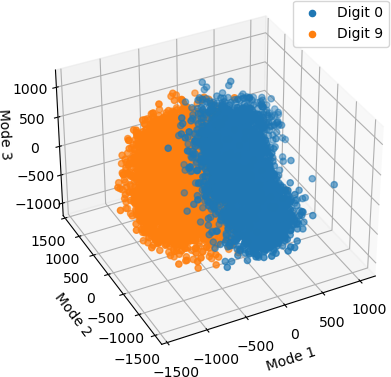
\includegraphics[width=0.4\textwidth]{modes_3d_09}\quad\quad\quad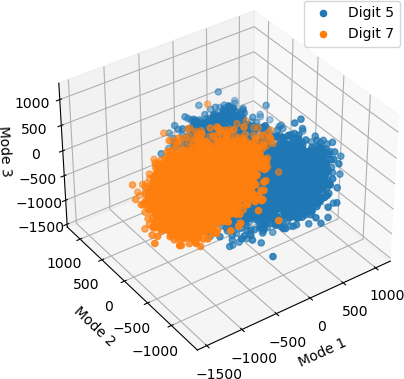
\includegraphics[width=0.4\textwidth]{modes_3d_57}
  \caption{Projections of the eigendecomposition coefficients onto the first three principal modes for training realizations classified as 0 and 9 (left) and 5 and 7 (right). This reveals that, from the perspective of these three modes, digits 0 and 9 are well-separated (particularly in mode 1) while digits 5 and 7 have significant interpenetration in this particular projection. In the higher mode space digits 5 and 7 are better separated.}\label{sep}
\end{figure}

As seen in Fig. \ref{sep}, projected onto the first three modes, the expansion coefficients of each image form clusters in the mode space. This geometric property means the classifiers described in Ref. \ref{class_sec}, which divide the eigenspace into separated groups with boundaries, and predict with these boundaries, will work well for digit classification. Importantly, this geometric separation occurs in the eigenspace, or principal components, of the digit images. Finally, the classifiers were applied in the following manner. First, classification of all pairs of two digits were tested using all three described methods. Second, three-digit classification was tested using LDA only. The following section describes the results obtained with the linear classifiers.

\section{Computational Results}
The first result tested was the LDA on all pairs of digits, shown in Fig. \ref{lda}. Easily-separated digits are seen to be 0 and 1, and 6 and 7. However, difficult-to-separate digits are 9 and 4, as well as 3 and 7. These easy and difficult to separate pairs are nicely explained by their disparities and similarities in pattern.

\begin{figure}[hb!]
  \centering
  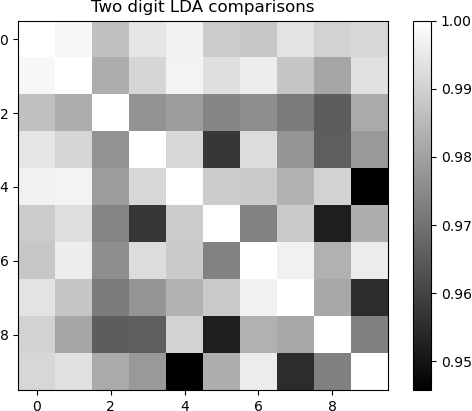
\includegraphics[width=0.4\textwidth]{2dgt_error_lda_50modes}\quad\quad\quad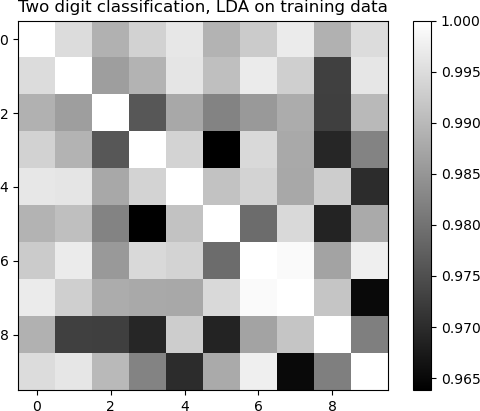
\includegraphics[width=0.4\textwidth]{ontrainingdata/lda_allmodes}
  \caption{Classification score of LDA method on digit pairs. (Left:) scores of the test data using 50-mode reduced training data. While all scores are $>94$\%, 2 has a poor trend and certain pairings are not good.\\(Right:) Classifier score on its own training data without dimension reduction, showing inherent LDA error.}\label{lda}
\end{figure}

\begin{figure}[ht!]
  \centering
  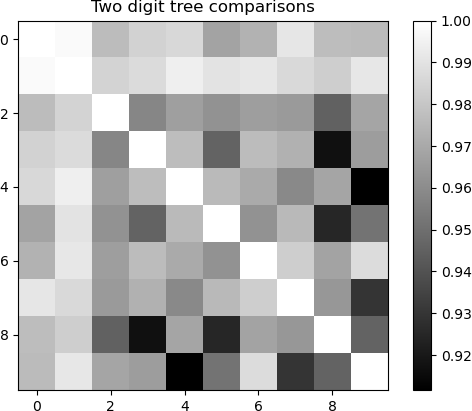
\includegraphics[width=0.4\textwidth]{2dgt_tree_50modes}\quad\quad\quad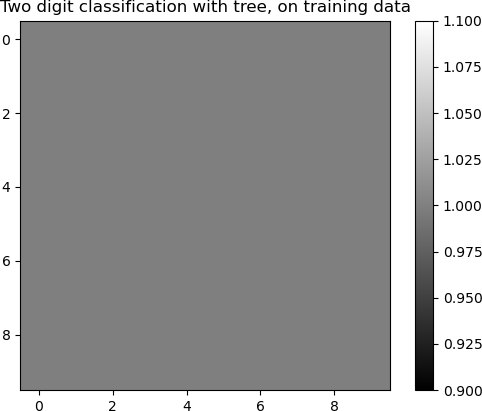
\includegraphics[width=0.4\textwidth]{ontrainingdata/tree_training}
  \caption{(Left:) Two-digit classification results using the decision tree method. Interestingly, larger errors are observed compared to the LDA, but the digit 2 consistently performs better. Errors on the difficult-to-distinguish pairs of the LDA are exacerbated by the decision tree. (Right:) The tree, at least with default settings, predicts its own training data exactly (so the colorbar was autoset). This indicates overfitting.}\label{tree}
\end{figure}

Further, predicting the original training data reveals the very same error pattern, though at a lower rate of incidence. This demonstrates an inherent error in the LDA method due to outliers, even though it operates on a minimized Rayleigh quotient. Now Fig. \ref{tree} demonstrates results with the decision tree method. The main takeaway from these results is that errors on difficult-to-distinguish data are made even worse by the decision tree compared to the LDA, but it predicts its own training data very well.

Next, the support vector machine was explored with results in Fig. \ref{svm}. The SVM was observed to be calculated faster than the decision tree \textit{and} to have accurate results to within almost 1\%! However, it has a small rate of error in predicting its own training data. As before, the SVM was trained on a 50-mode reduced dimension eigenprojected dataset. Comparison of Figs. \ref{lda}, \ref{tree}, and \ref{svm} shows that all three methods distinguish 0 and 1 very well, and all have the most difficulty with 4 and 9. However, the SVM classifier predicts with great accuracy and beats the others by several percentage points.

It must be stressed that this analysis is done deterministically on a single set of training and test data. Generally speaking these methods are to be cross-validated by randomly sampling a subset of the training data and doing a statistical analysis of the resulting scores for different training set sizes. The author played around with this a bit while doing the assignment but did not include these results for brevity. The general trend was that scores were lower when using a smaller training set, but the SVM still did the best.

\begin{figure}[hb!]
  \centering
  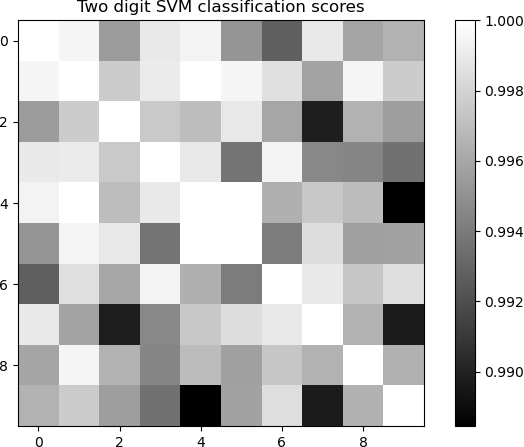
\includegraphics[width=0.4\textwidth]{2dgt_svm_50modes}\quad\quad\quad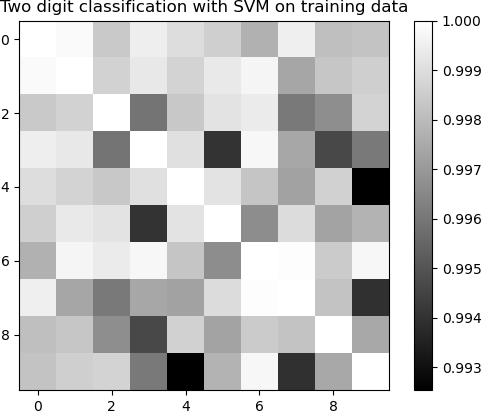
\includegraphics[width=0.4\textwidth]{ontrainingdata/svm_training}
  \caption{Two-digit classification results with the SVM method. The support vector technique is seen to be the best of the three methods overall, and intriguingly has almost perfect discernment between digits 4 and 5. It stumbles most on 4 and 9, however perhaps even a human would on these digits when handwritten.}\label{svm}
\end{figure}

\begin{figure}[ht!]
  \centering
  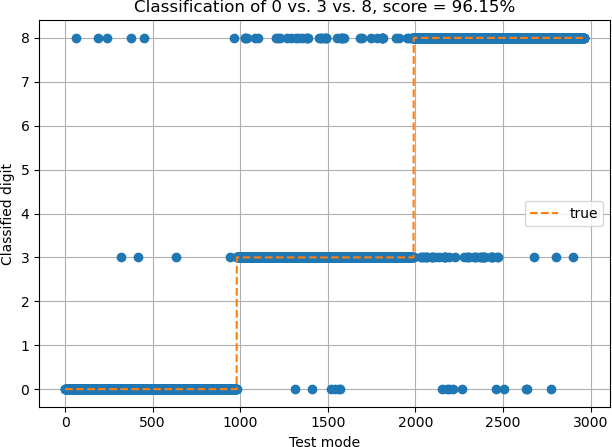
\includegraphics[width=0.315\textwidth]{lda3/3digit_lda_038}\quad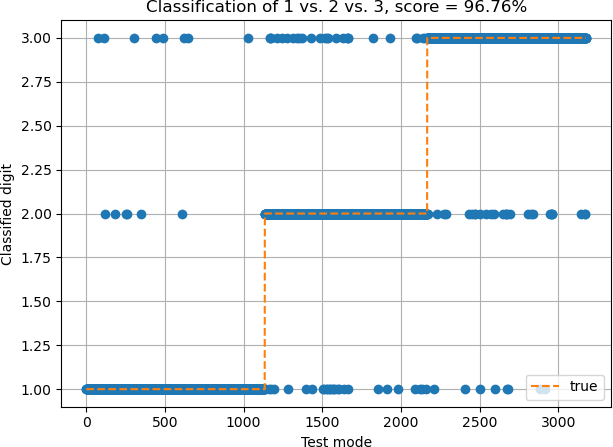
\includegraphics[width=0.315\textwidth]{lda3/3digit_lda_123}\quad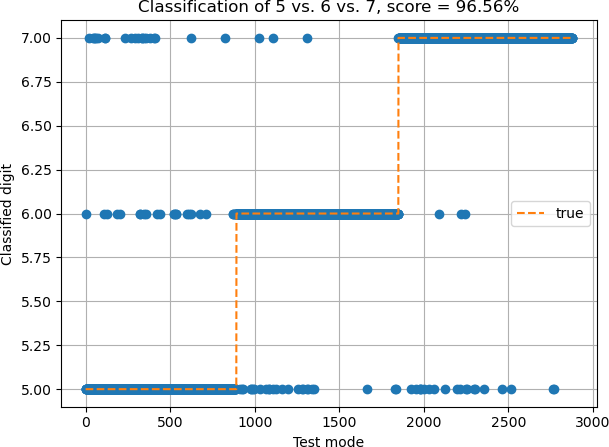
\includegraphics[width=0.315\textwidth]{lda3/3digit_lda_567}
  \caption{Simultaneous classification of three digits using LDA on the sets of digits 038, 123, and 567. Generally good classification in line with the ``worst'' results of the two-digit LDA is observed, here $> 96$\%.}\label{threedigit}
\end{figure}

\subsection{Three-digit classification}
As an initial exploration of further capabilities, Fig. \ref{threedigit} shows LDA applied to categorize three digits simultaneously. Good results are seen in these cases, with general trends in line with the results of the two-digit LDA in Fig. \ref{lda}. However, one would expect that simultaneous classification of all nine digits would run into issues due to the general mixing of eigenvalues for the difficult pairs such as 9 and 4, contaminating performance of the entire classification scheme. Three digits was generally seen to work well though.

% \begin{figure}[h]
%   \centering
%   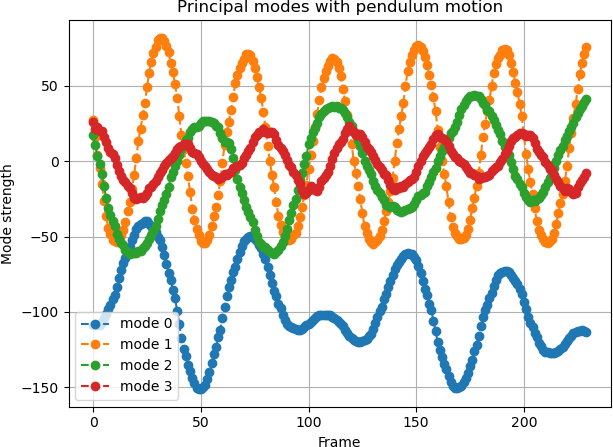
\includegraphics[width=0.45\textwidth]{pca_pend2}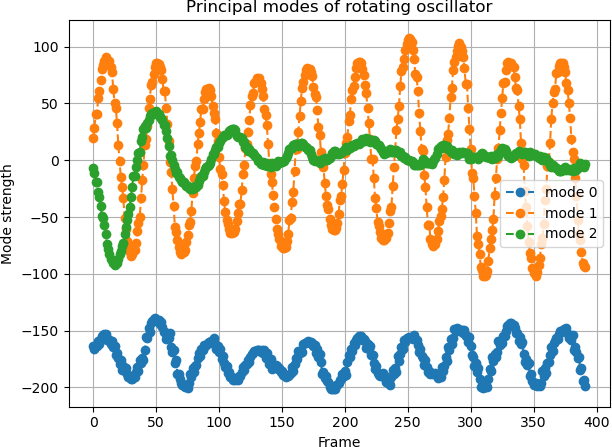
\includegraphics[width=0.45\textwidth]{pca_rotate2}
%   \caption{Projected modes of bucket coordinates for cases of SHM superimposed on pendulum motion (left) and bucket rotation (right). In comparison to the baseline case (Fig. \ref{sns}) clearly ``mode 1'' still describes the bucket SHM as their frequencies match. The pendulum motion appears as a lower-frequency oscillation apparently in ``mode 2''. However, the occurence of both oscillations appears to leave a modulated trace (superposition?) in mode 0, in curious correlation with the Wigner function experiments of the last homework. The rotating oscillator case shows a damped rotation tendency in ``mode 2,'' matching the video here.}\label{pr}
% \end{figure}

% \begin{figure}[hb!]
%   \centering
%   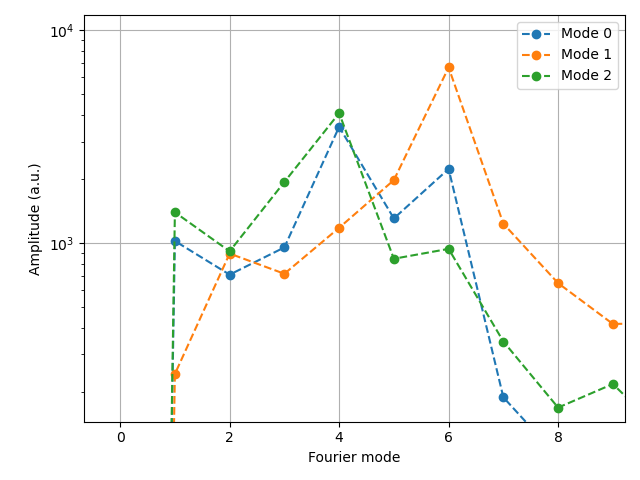
\includegraphics[width=0.5\textwidth]{pendulum_fft3}
%   \caption{First few Fourier components from FFT of the pendulum case, showing the frequencies in the ``mode 0'' waveform to be the SHM and pendulum frequencies 4 and 6, and perhaps interference in mode 5.}\label{pend_fft}
% \end{figure}

% \begin{table}[b]
%   \centering
%   \begin{tabular}{|l|l|l|l|l|l|l|l|l|}
%     \hline
%     Time {[}hr{]}   & 0-3.5 & 3.5-7.0 & 7.0-10.5 & 10.5-14.0 & 14.0-17.5 & 17.5-21.0 & 21.0-24.5 & All-time average \\ \hline
%     $\langle k_x\rangle_T$ {[}1/L{]} & 0.814 & 0.661   & 0.784    & 0.760     & 0.810     & 0.728     & 0.802     & 0.766            \\ \hline
%     $\langle k_y\rangle_T$ {[}1/L{]} & 0.271 & 0.292   & 0.331    & 0.240     & 0.341     & 0.267     & 0.271     & 0.288            \\ \hline
%     $\langle k_z\rangle_T$ {[}1/L{]} & -1.00 & -1.03   & -1.09    & -1.06     & -1.13     & -1.07     & -1.1125   & -1.07            \\ \hline
%   \end{tabular}
%   \caption{Observed center frequencies of data following spectral averaging over time intervals of $3.5$ hours, with seven samples per interval, then used as the filter frequencies $k_0$ in the Gaussian filter. The arbitrary spatial unit is given as $L$, not to be confused with domain length. The all-time average is given as well.}\label{frequencies}
% \end{table}

% Note that in Table \ref{frequencies} negative wavenumbers are used as the given spatial data is complex, meaning that the reality condition is not satisfied, instead $\hat{f}(-k) = \hat{f}^*(k)$ in this dataset. The absolute value is reported as ``the frequency'' of the submarine, however. This identifies the submarine's spectral signature as $\bm{k} \approx \{0.766 \pm 0.05, 0.288 \pm 0.03, 1.07 \pm 0.04 \}$ {[}1/L{]} by mean and standard deviation of the window averages of Table \ref{frequencies}, where L is an arbitrary space unit corresponding to that of the provided data, \textit{not} the domain length. The width of the space or frequency ``submarine Gaussian'' was not measured for ease of analysis.

% Having computed the center frequencies, the spectrum was filtered and the trajectory determined according to the schematic Steps 4 and 5. The resulting 3D trajectory and top-down position given in Figs. \ref{traj:3d}, \ref{traj:2d} respectively. This suggests the submarine is currently located around $\bm{x}\sim(-5, 6.5)$ in $(x,y)$.

% \begin{figure}[hb]
%   \centering
%   \begin{subfigure}{0.42\textwidth}
%     \centering
%     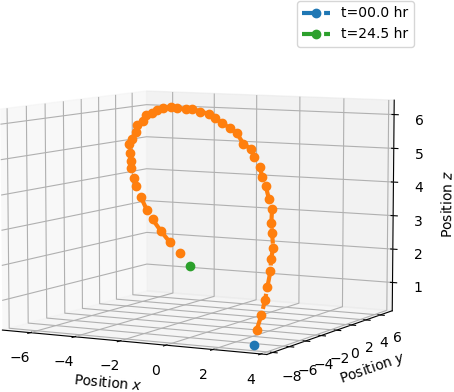
\includegraphics[width=0.99\linewidth]{pics/3d_traj}
%     \caption{Three-dimensional trajectory of submarine, showing a rise and dive maneuver.}\label{traj:3d}
%   \end{subfigure}
%   \begin{subfigure}{0.42\textwidth}
%     \centering
%     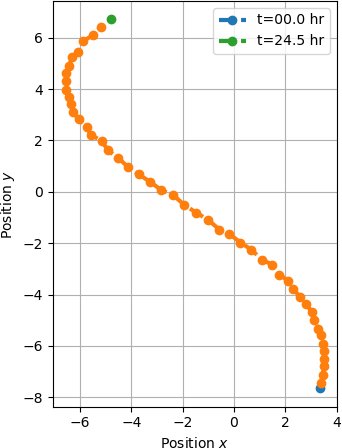
\includegraphics[width=0.6\linewidth]{pics/2d_traj}
%     \caption{Top-down view of predicted trajectory. Ideal search area for submarine-tracking aircraft is around $\bm{x} \sim (-5, 6.5)$ and continuing north-east.}\label{traj:2d}
%   \end{subfigure}
%   \caption{Identified submarine trajectory sampled 49 times in a 24.5 hour period, in 3D and 2D projections.}
% \end{figure}

% Summary and Conclusions
\section{Summary and Conclusions}
This numerical experiment examined three types of linear classifiers: linear discriminant analysis, decision tree, and support vector machine. The decision tree was observed to overfit the data, however tweaking its settings would probably reduce that effect. An initial dive into this by constraining the number of leaf nodes showed a relaxation of the overfitting, but not really an improvement in its scores.

Principal component analysis was used to formulate a well-separated parameter space in terms of eigendecomposition coefficients and dimensionality reduction was experimented with, using truncated characteristic mode expansions. The support vector machine was seen to be the very best method of those examined here. As usual, Python was used for all implementations in this exercise and may be found at the author's Github page \href{https://github.com/crewsdw/amath582}{here} along with some cool movies of the eigenexpansions converging.

% % References
\bibliographystyle{unsrt}
\bibliography{references}

% % Appendices
\begin{appendices}

% \newpage
% % MATLAB Functions
\section{Python Functions}\label{functions}
The following list compiles important Python functions used in implementation:
\begin{itemize}
\item The all-important masking capability \texttt{array[bool condition] = x} is used to identify labelled data,
\item The \texttt{sklearn} package was used for classifier capabilities, including the subroutines
  \begin{itemize}
  \item \texttt{sklearn.discriminant\_analysis} with class \texttt{LinearDiscriminantAnalysis},
  \item \texttt{sklearn.tree} with class \texttt{DecisionTreeClassifier},
  \item \texttt{sklearn} with class \texttt{svm} (for SVM).
  \end{itemize}
\item For each classifier package, one trains using \texttt{model.fit(data, labels)} and predicts\\ using \texttt{P = model.predict(test)}.
\end{itemize}

% % MATLAB Codes
\section{Python Implementation}\label{implementation}
% A separate analysis script was used for each dataset and the files are quite similar. Only pendulum is shown for brevity (see Github page for other files).
% % Wigner function file \texttt{fourier.py}:
% \lstinputlisting{wpendulum.py}
% \vspace{5cm}
Main implementation file \texttt{hw4.py}:
\lstinputlisting{hw4.py}
% \begin{listing}[h]
% \inputminted{matlab}{example.m}
% \caption{Example code from external file.}
% \label{listing:examplecode}
% \end{listing}

\end{appendices}

\end{document}